\subsection{MLOps Components \& Architecture}

\begin{figure}[h]
    \centering
    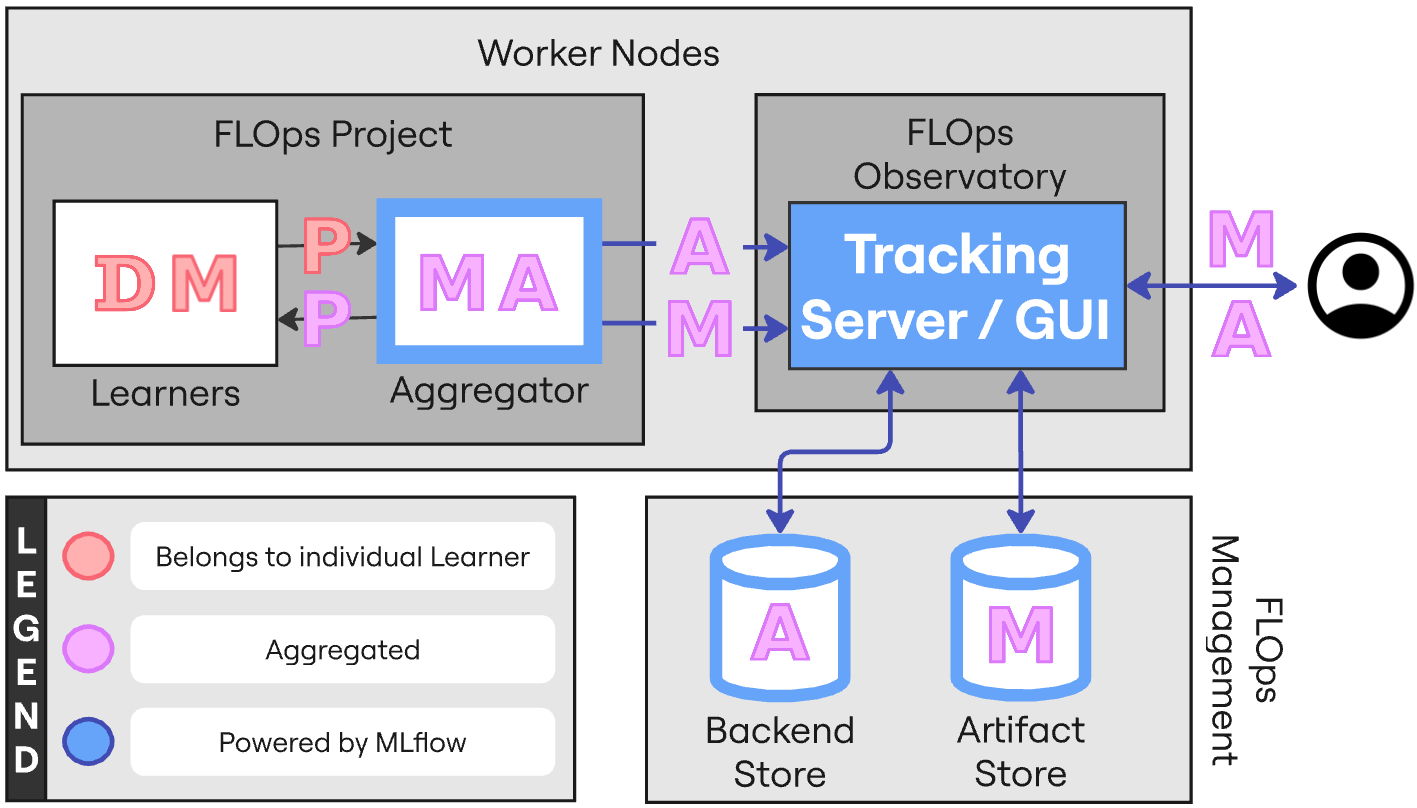
\includegraphics[width=1.0\textwidth]{mlops_components.png}
    \caption{FLOps' MLOps Architecture}
    \label{fig:mlops_architecture}
\end{figure}

This subsection builds on top of the discussed MLflow background (\ref{subsection:mlflow}) and subsystem decomposition (\ref{subsection:subsystem_decomposition}).

Figure \ref{fig:mlops_architecture} shows FLOps' MLOps architecture.
MLflow powers many FLOps' MLOps capabilities.
After every training round, the aggregator logs lightweight artifacts like metrics, parameters, tags, or runs.
In addition, the aggregator stores exactly one global model copy locally.
After every round, the aggregator checks if the new model's performance is better or worse.
The aggregator will update its local model if the new model is better.
At the end of the last training round, the aggregator sends the best trained global model to the artifact store.

An MLflow run represents an individual execution of (usually ML) code.
Each run can collect various pieces of information, such as metrics, hyperparameters, or custom tags.
These lightweight elements are represented as A in the Figure.
An MLflow experiment gathers multiple runs.
FLOps maps these MLflow terms directly to FL.
An experiment becomes an FLOps project and runs are FL training rounds.

The aggregator logs everything besides local elements over the tracking server. 
The tracking server works as a proxy for artifacts.
Thus, any access to any logged objects goes through the tracking server.
The tracking server itself does not have any state.
Its GUI showcases the stored elements in the backend and artifact stores hosted via the FLOps management.
Note that these stores can be deployed and scaled individually onto different machines.
There are various ways of setting up and provisioning MLflow components.
For example, the backend store can be a local directory, a remote database, a cloud file server, or blob storage.
The backend store hosts lightweight elements, and the artifact store hosts heavy-weight elements such as models or images.
FLOps currently uses a MySQL database for the backend store and a vsftpd (very secure FTP daemon) server for the artifact store.

It is noteworthy that no MLOps logging takes place on the learners.
Only the aggregator uses these techniques.
This approach works as expected regarding concrete FL metrics and models.
MLflow also provides a way to track system metrics, which FLOps uses.
These metrics only capture information about the aggregator, not the connected learners.
No information belonging to individual learners gets logged.
Furthermore, FLOps ensures that users can only access their own recorded artifacts.
FLOps explicitly upholds these separations to minimize possible privacy hazards and attack vectors.